\documentclass[a4paper]{article}

\usepackage{tikz}
\usepackage{pgfplots}
\usepackage{libertine}
\usetikzlibrary{patterns}

\pgfplotsset{compat=1.4} 
\pagestyle{empty}

\definecolor{bblack}{HTML}{111111}
\definecolor{wwhite}{HTML}{C8C8C8}

\makeatletter
\tikzset{nomorepostaction/.code=\let\tikz@postactions\pgfutil@empty}
\makeatother


\begin{document}

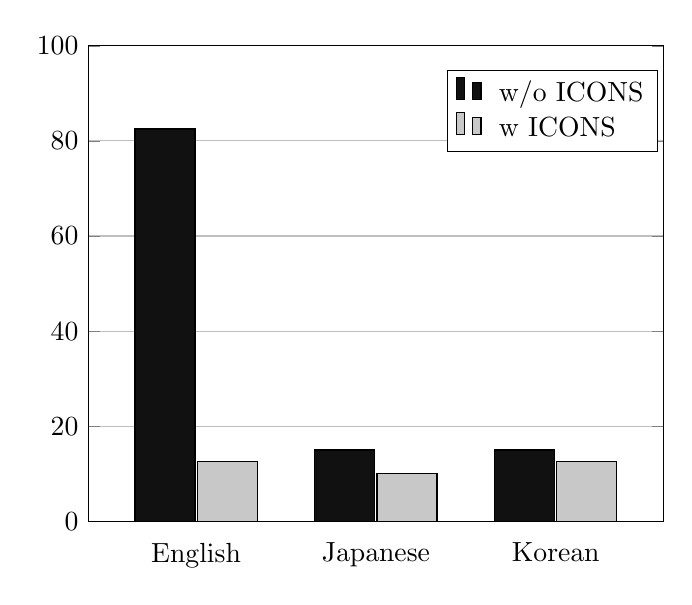
\begin{tikzpicture}
    \begin{axis}[
        width=3.5in,
	height=3in,
        major x tick style = transparent,
        ybar=2*\pgflinewidth,
        ymajorgrids = true,
        symbolic x coords={English,Japanese,Korean},
        xtick = data,
        scaled y ticks = false,
        enlarge x limits=0.3,
	ymin=0, ymax=100,
        legend cell align=left,
        legend style={
                at={(0.99,0.95)},
                anchor=north east,
                column sep=1ex
        }
    ]
  \addplot[style={bar width=0.3in,fill=bblack,draw=black}]
            coordinates {	(English,82.5)
				(Japanese,15.0)
				(Korean,15.0)    };
  \addplot[style={bar width=0.3in,fill=wwhite,draw=black}]
            coordinates {	(English,12.5)
				(Japanese,10.0)
				(Korean,12.5)    };
 \legend{w/o ICONS,w ICONS}
 \end{axis}
\end{tikzpicture}
\end{document}




